\section{System Architecture}
\subsection{Components and their responsibilities}

\underline{\textbf{Registration}}\\
\textbf{Signup - }Prompts the user to enter the required fields according to the user type. And validate them with the help of User verification component.\\
\textbf{User verification - } Verifies the user account by providing data to the Admin component.\\
\textbf{User creation - } Creates user accounts once the User verification component provides the necessary data, or provides an error message if the verification fails.\\

\underline{\textbf{Login}}\\
\textbf{Login - }Gets login credentials from the user and gets those credentials verified from User Authentication component and redirects the user to the respective user interface or provides error messages if the credentials are wrong.\\
\textbf{Forgot password - }Let the user reset his forgotten password by entering his email address. The component checks the given username with the User Authentication component and then sends the password reset email if the email or username is verified. Otherwise, it displays the relevant error messages.\\
\textbf{User authentication - }Verifies user credentials in login and password reset processes. It uses the user table from the database to verify the credentials given by the user.\\

\underline{\textbf{Admin}}\\
\textbf{Admin dashboard - }This UI component of the admin shows the functionalities that the admin can perform. Furthermore, it shows a few statistics of the overall system as well.\\
\textbf{Manage guides - }Let the admin manage, delete guide profiles, and see their guidance history.\\
\textbf{Manage rental services - }Let the admin manage, delete rental services, and see their performance history.\\
\textbf{Resolve complaints - }Let the admin resolve complaints made by customers, rental services, guides, and pass the data to the relevant components of the said users.\\
\textbf{Manage tips and knowhows - }Let the admin insert, delete, and update blogs.\\
\textbf{User verification - }Verifies the user accounts as requested by the Sign-up subsystem, and sends results.\\
\textbf{Report generation - }Generates reports of selected data and performance as desired.\\

\underline{\textbf{Customer}}\\
\textbf{Customer Dashboard - }This UI component of the customer shows the functionalities that the customer can perform. Furthermore, it shows a few statistics of the customer such as past guide hiring, and equipment bookings as well.\\
\textbf{Equipment booking - }Let the customer browse for equipment and book desired equipment.\\
\textbf{Guide hiring - }Let the customer search for guides and hire desired guides.\\
\textbf{Make complaint - }Let customers make complaints about a rental service and/or a guide, and send the necessary data to the Resolve complaint component of admin.\\

\underline{\textbf{Rental service }}\\
\textbf{Rental service dashboard - }This UI component of the rental service shows the functionalities that the rental service can perform. Furthermore, it shows a few statistics of the rental service such as past equipment bookings, and currently hired equipment as well.\\
\textbf{Equipment booking - }Handles equipment bookings done by the customers and keeps track of their payments.\\
\textbf{Equipment handling - }Adds and removes equipment, also updates equipment with the data provided by the Equipment booking Component.\\
\textbf{Make complaint - }Make complaints about customers.\\

\underline{\textbf{Guide}}\\
\textbf{Guide dashboard - }This UI component of the guide shows the functionalities that the guide can perform. Furthermore, it shows a few statistics of the guide such as past tours, and calendar availability as well.\\
\textbf{Manage guide packages - }Add, remove, and update guide packages.\\
\textbf{Manage calendar availability - }Updates the calendar availability according to the bookings done by customers.\\
\textbf{Guide booking - }Handles bookings done by the customers and keeps track of their payments.\\
\textbf{Make complaints - }Make complaints about customers.\\

\underline{\textbf{Tips and Know-hows}}\\
\textbf{Tips and know-hows - }This UI component shows the tips and know-hows to all users.\\
\textbf{Manage Tips and know-hows - }Manages tips and know-hows, with admin component.\\

\underline{\textbf{Payment - }}Handles the payments done by customer when booking equipment and hiring guides.\\



\subsection{Component interactions}

\begin{figure}[h!]
    \centering
    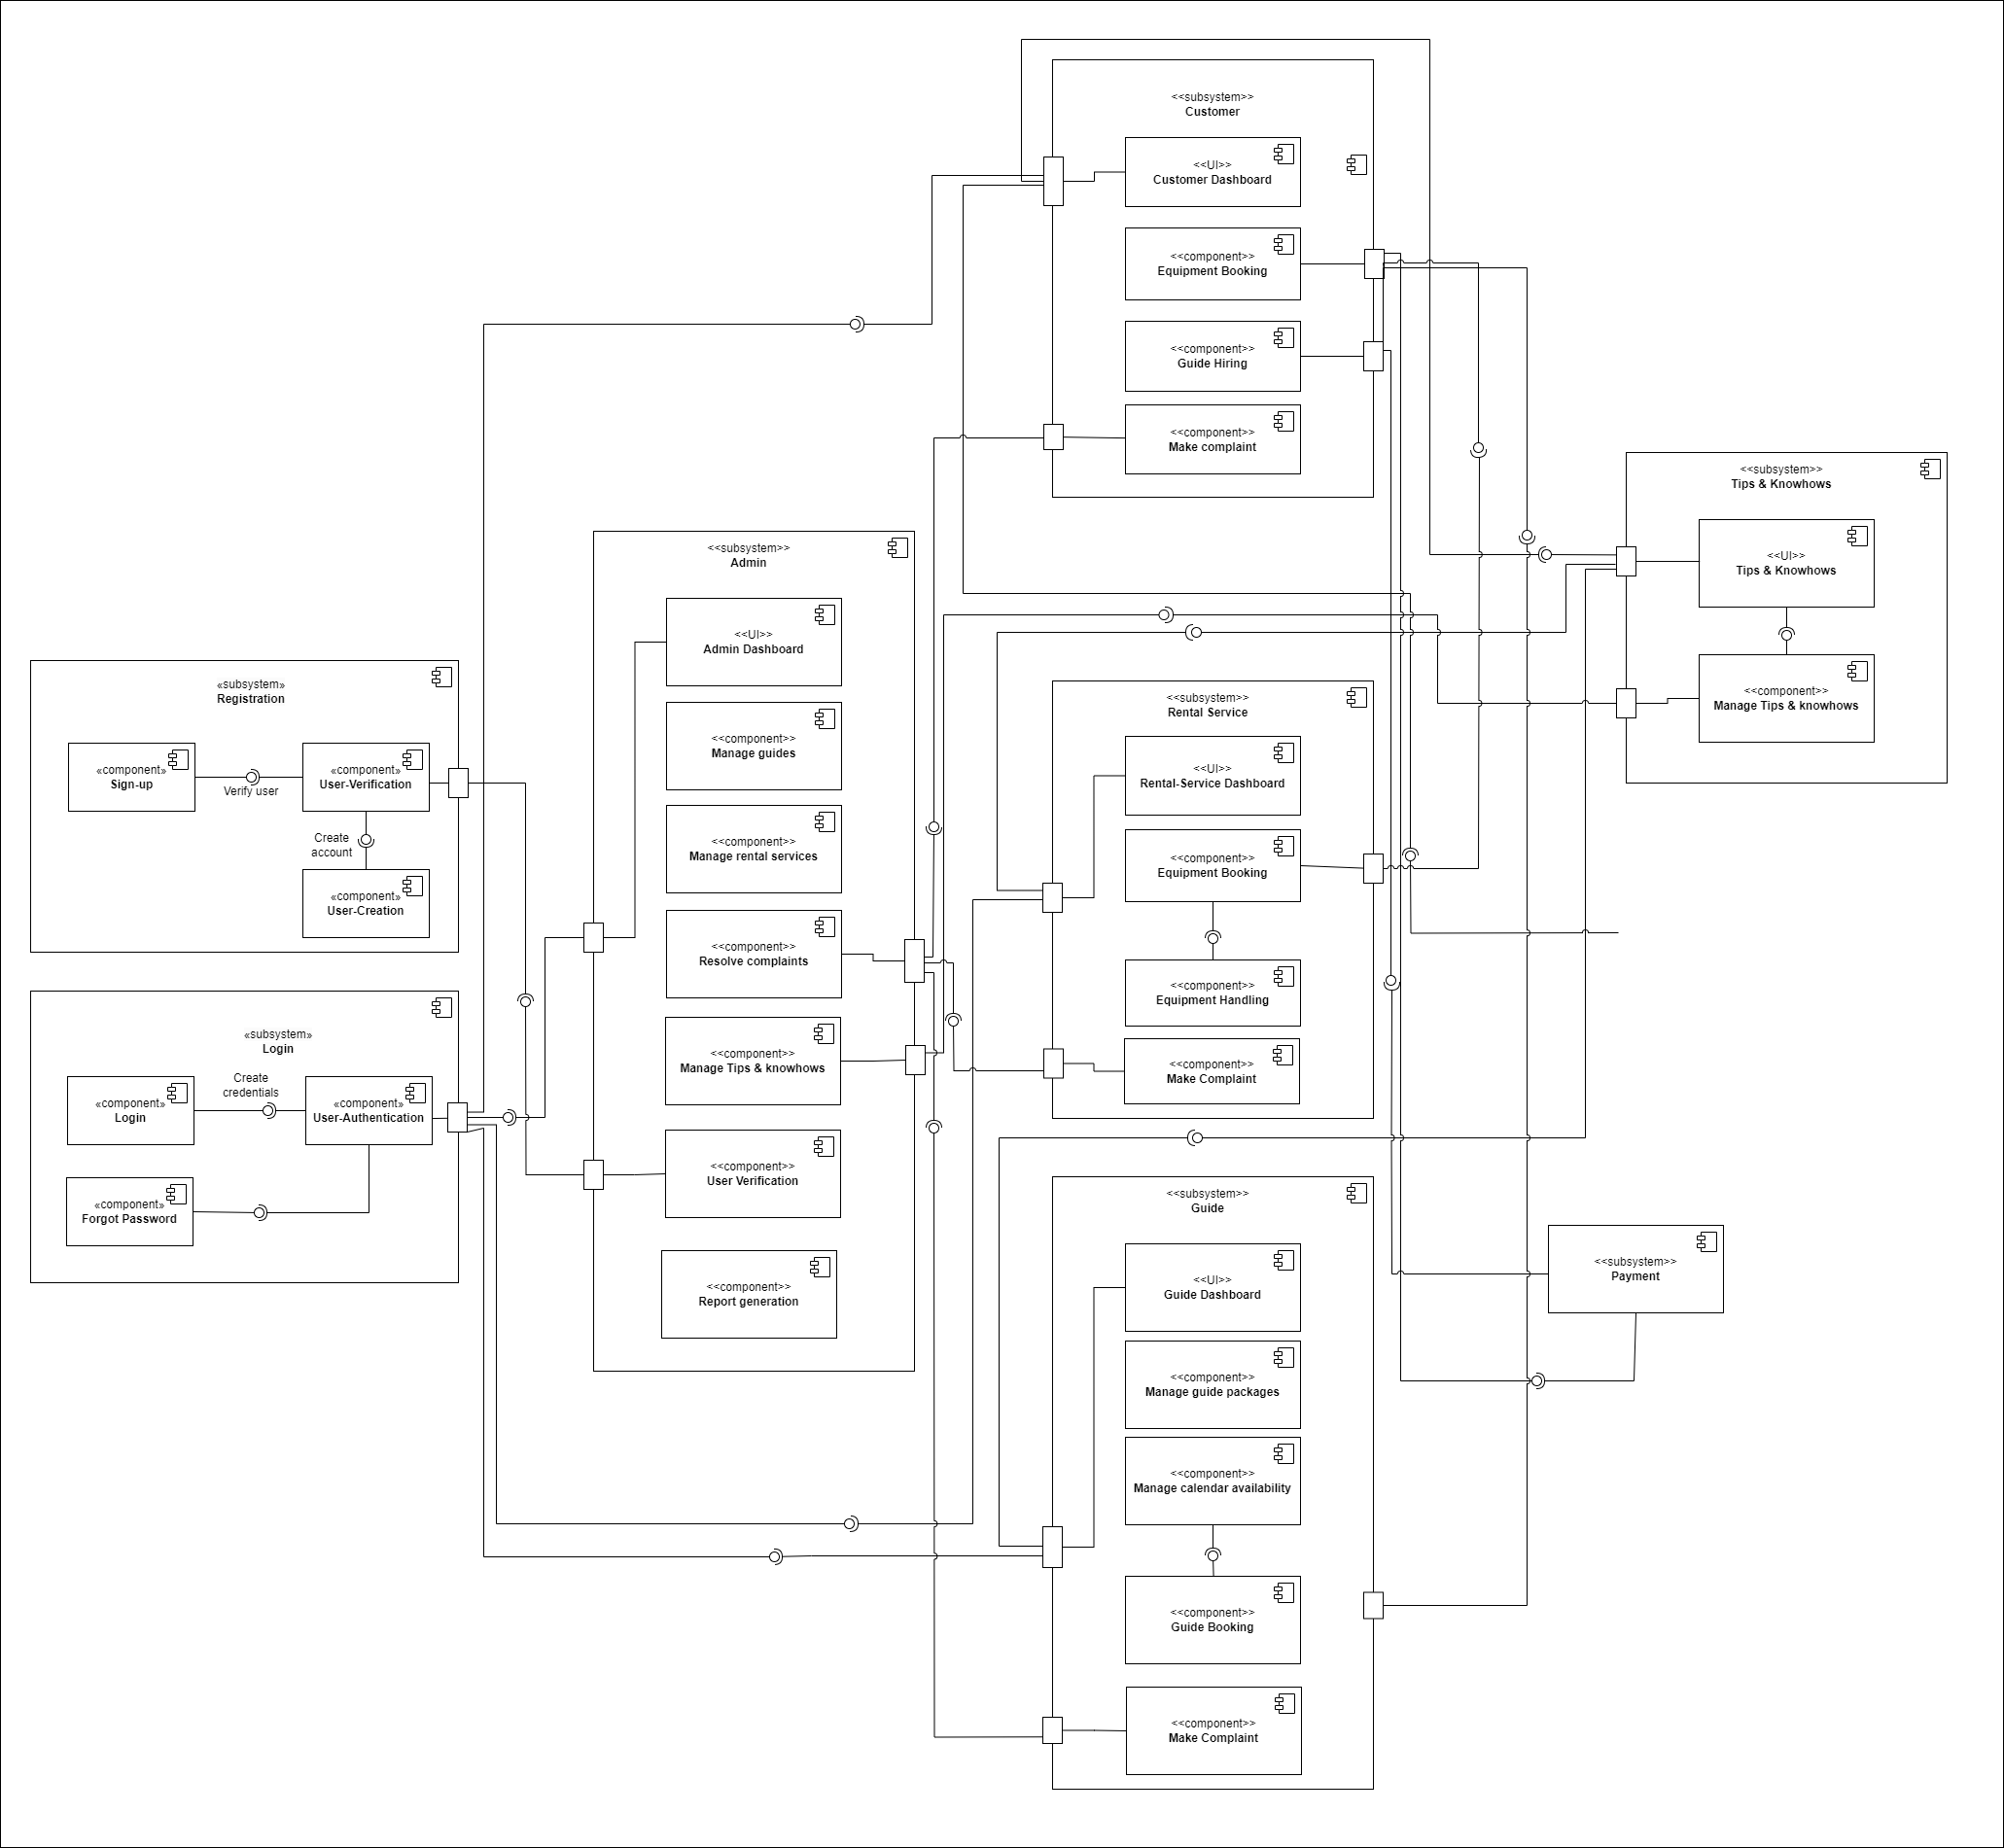
\includegraphics[width=1\textwidth]{Images/component.drawio.png}
    \caption{Component Diagram}
    \label{fig:enter-label}
\end{figure}
\clearpage